\section{Spectral Energy analysis specific to datasets}\label{app:Espectra}

\begin{figure}[H]
    \centering
    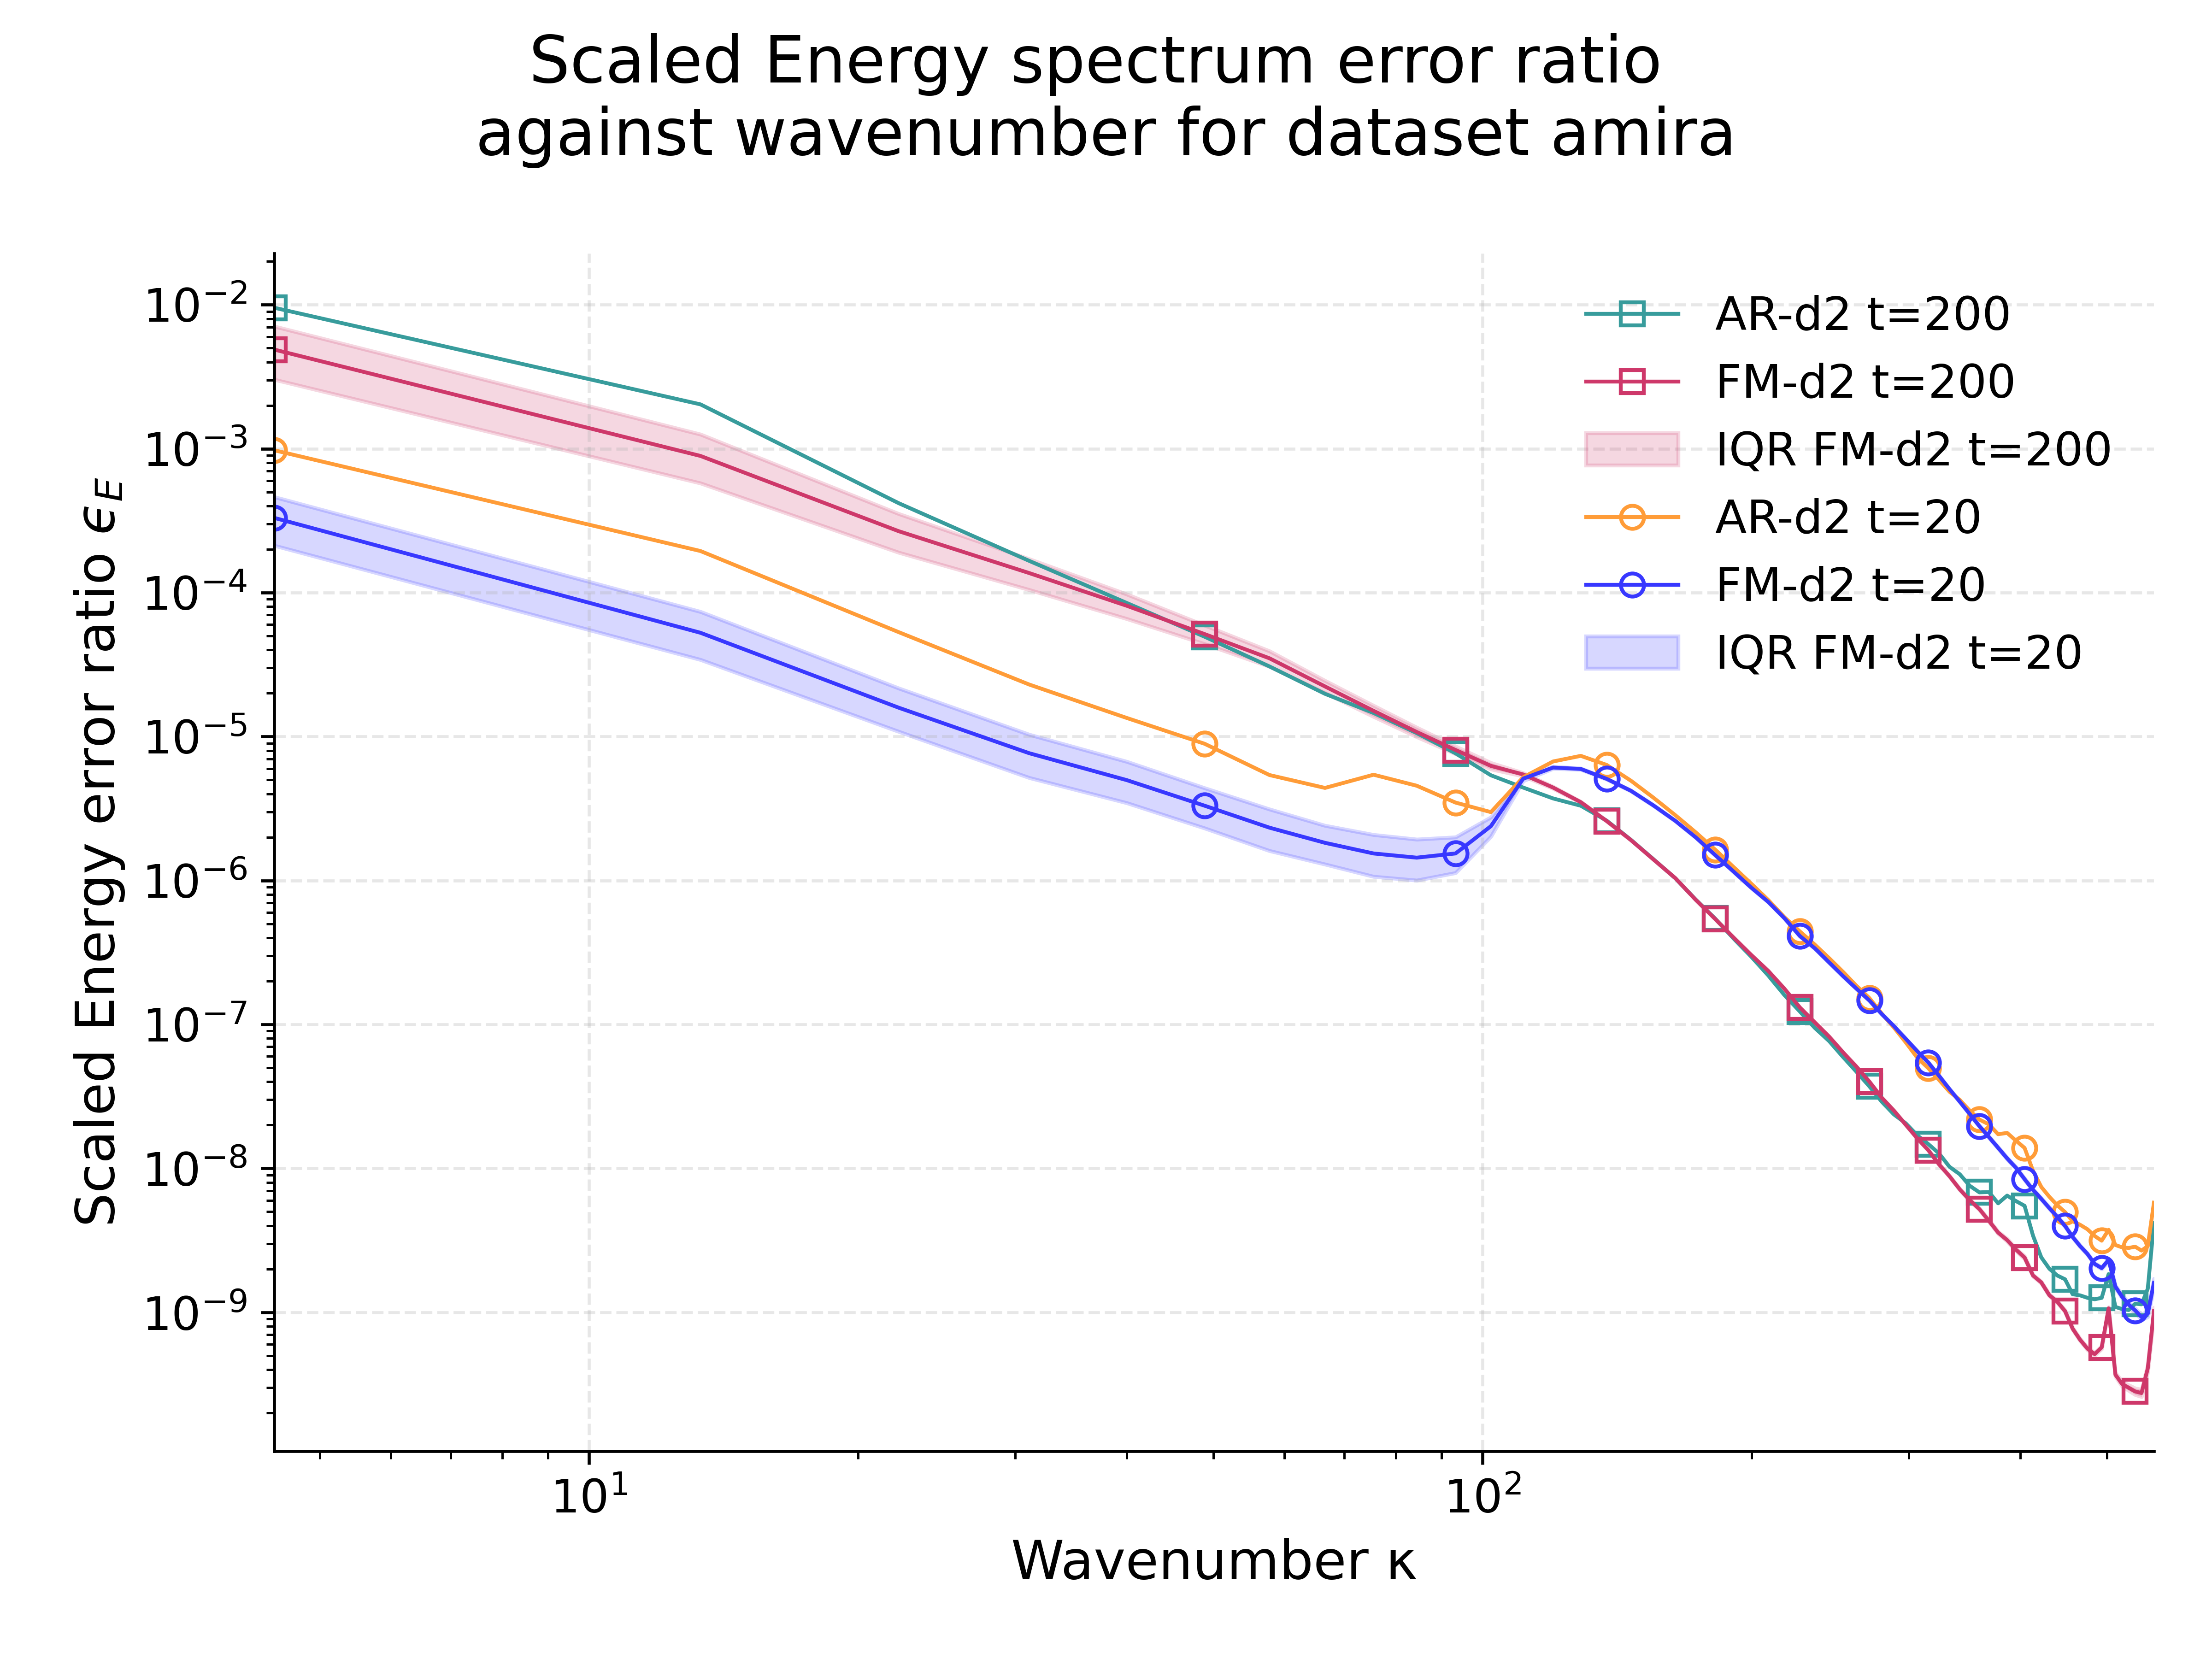
\includegraphics[width=0.8\textwidth]{figs/results/spectra/spectrum_E_amira.png}
    \caption{Scaled energy spectrum error ratio $\epsilon_E$ per wavenumber for the \texttt{amira} dataset, evaluated at $t=20$ and $t=200$.}
    \label{fig:appendix_spectrum_E_amira}
\end{figure}

\begin{figure}[H]
    \centering
    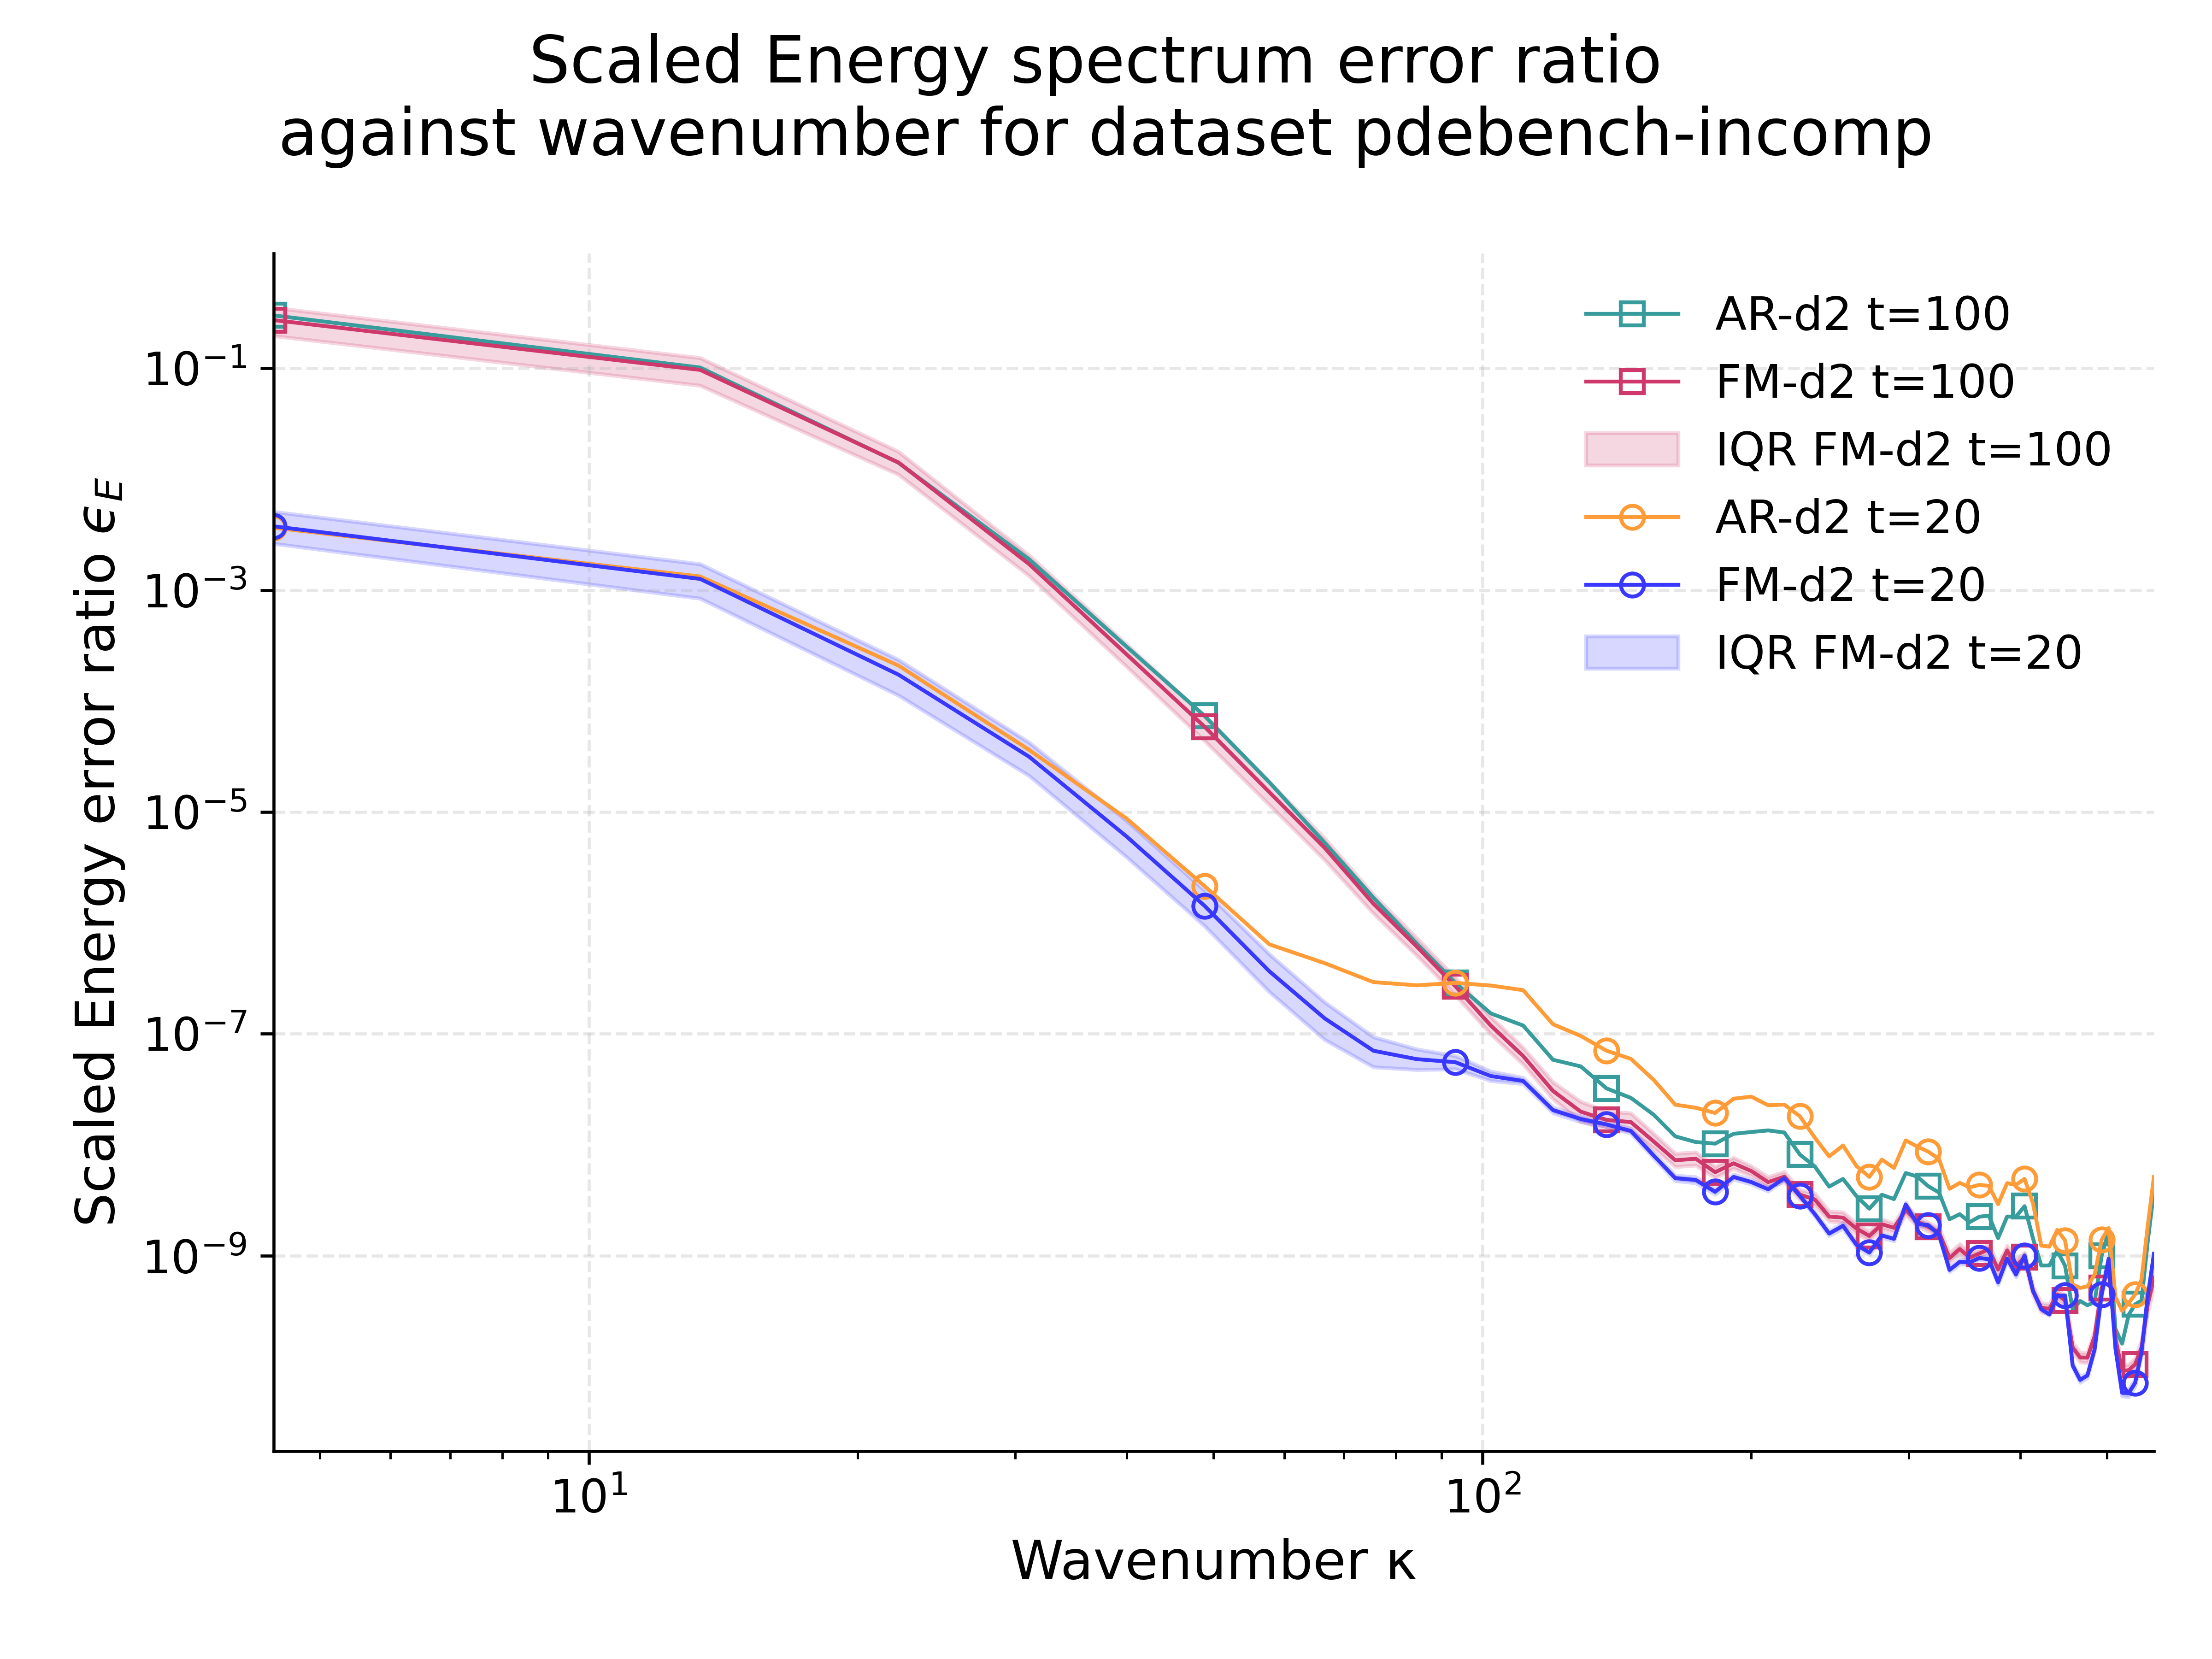
\includegraphics[width=0.8\textwidth]{figs/results/spectra/spectrum_E_pdebench-incomp.png}
    \caption{Scaled energy spectrum error ratio $\epsilon_E$ per wavenumber for the \texttt{pdebench-incomp} dataset, evaluated at $t=20$ and $t=100$.}
    \label{fig:appendix_spectrum_E_pdebench_incomp}
\end{figure}

\begin{figure}[H]
    \centering
    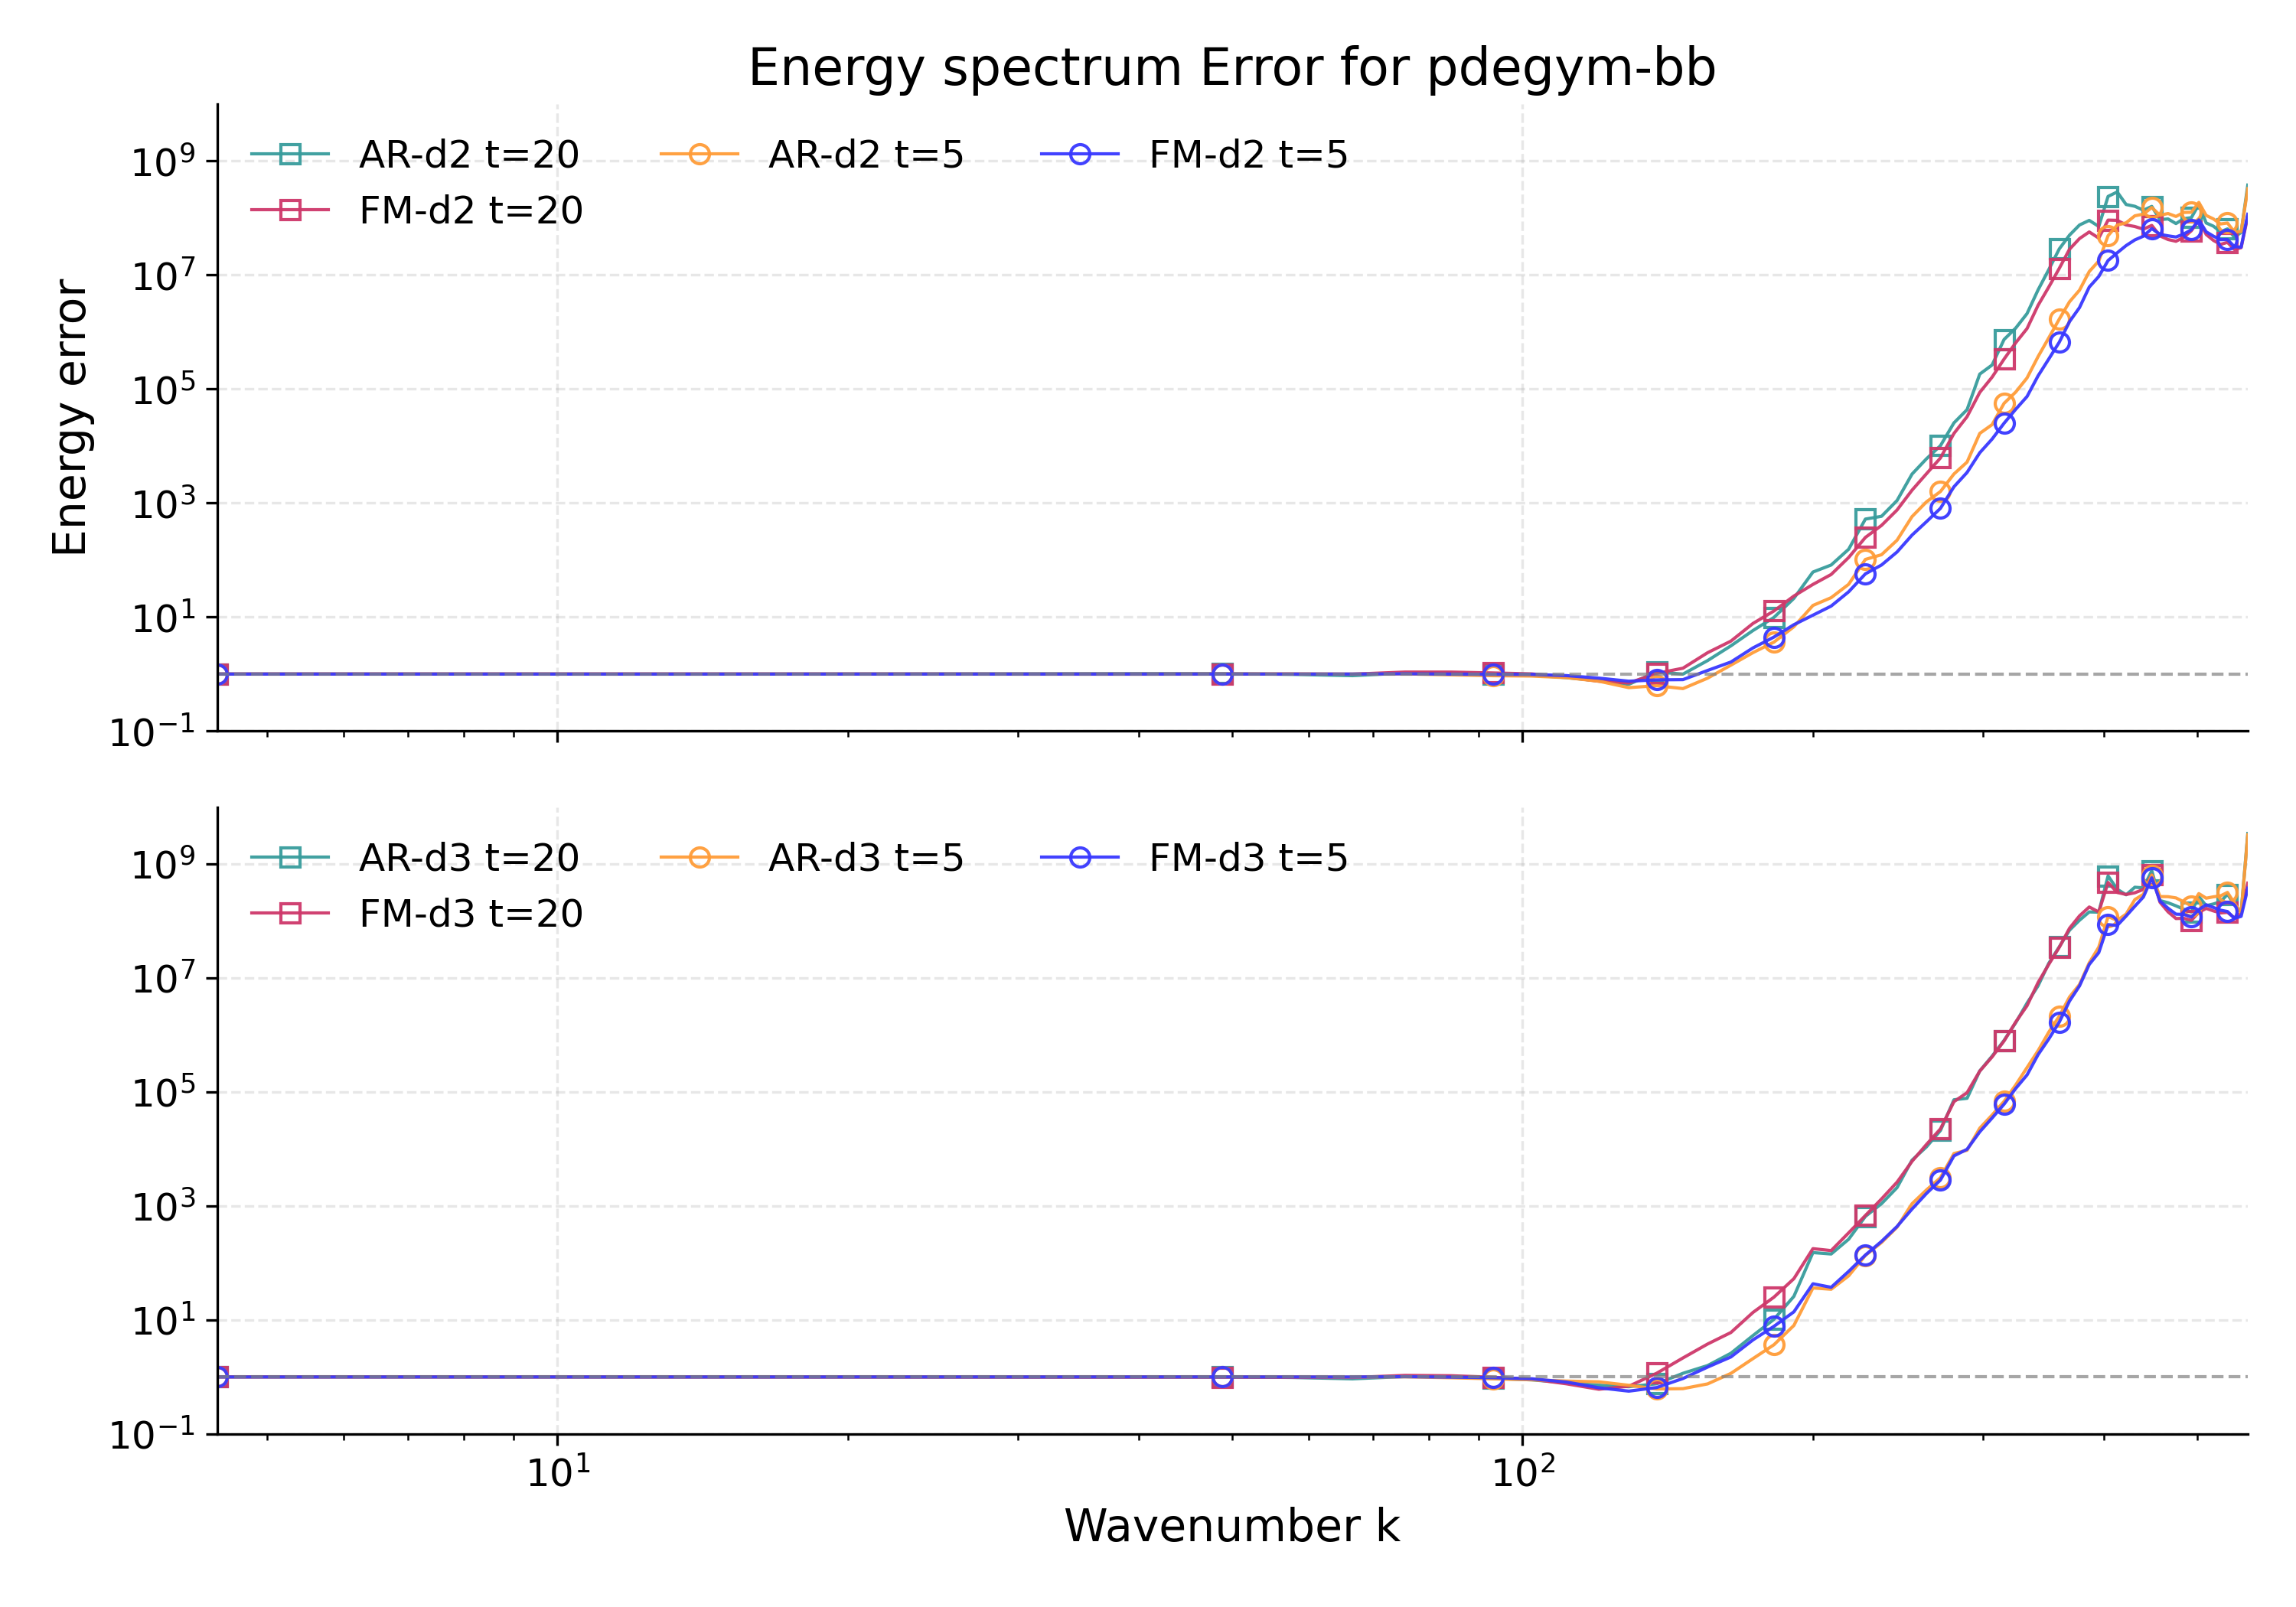
\includegraphics[width=0.8\textwidth]{figs/results/spectra/spectrum_E_pdegym-bb.png}
    \caption{Scaled energy spectrum error ratio $\epsilon_E$ per wavenumber for the \texttt{pdegym-bb} dataset, evaluated at $t=5$ and $t=20$.}
    \label{fig:appendix_spectrum_E_pdegym_bb}
\end{figure}

\begin{figure}[H]
    \centering
    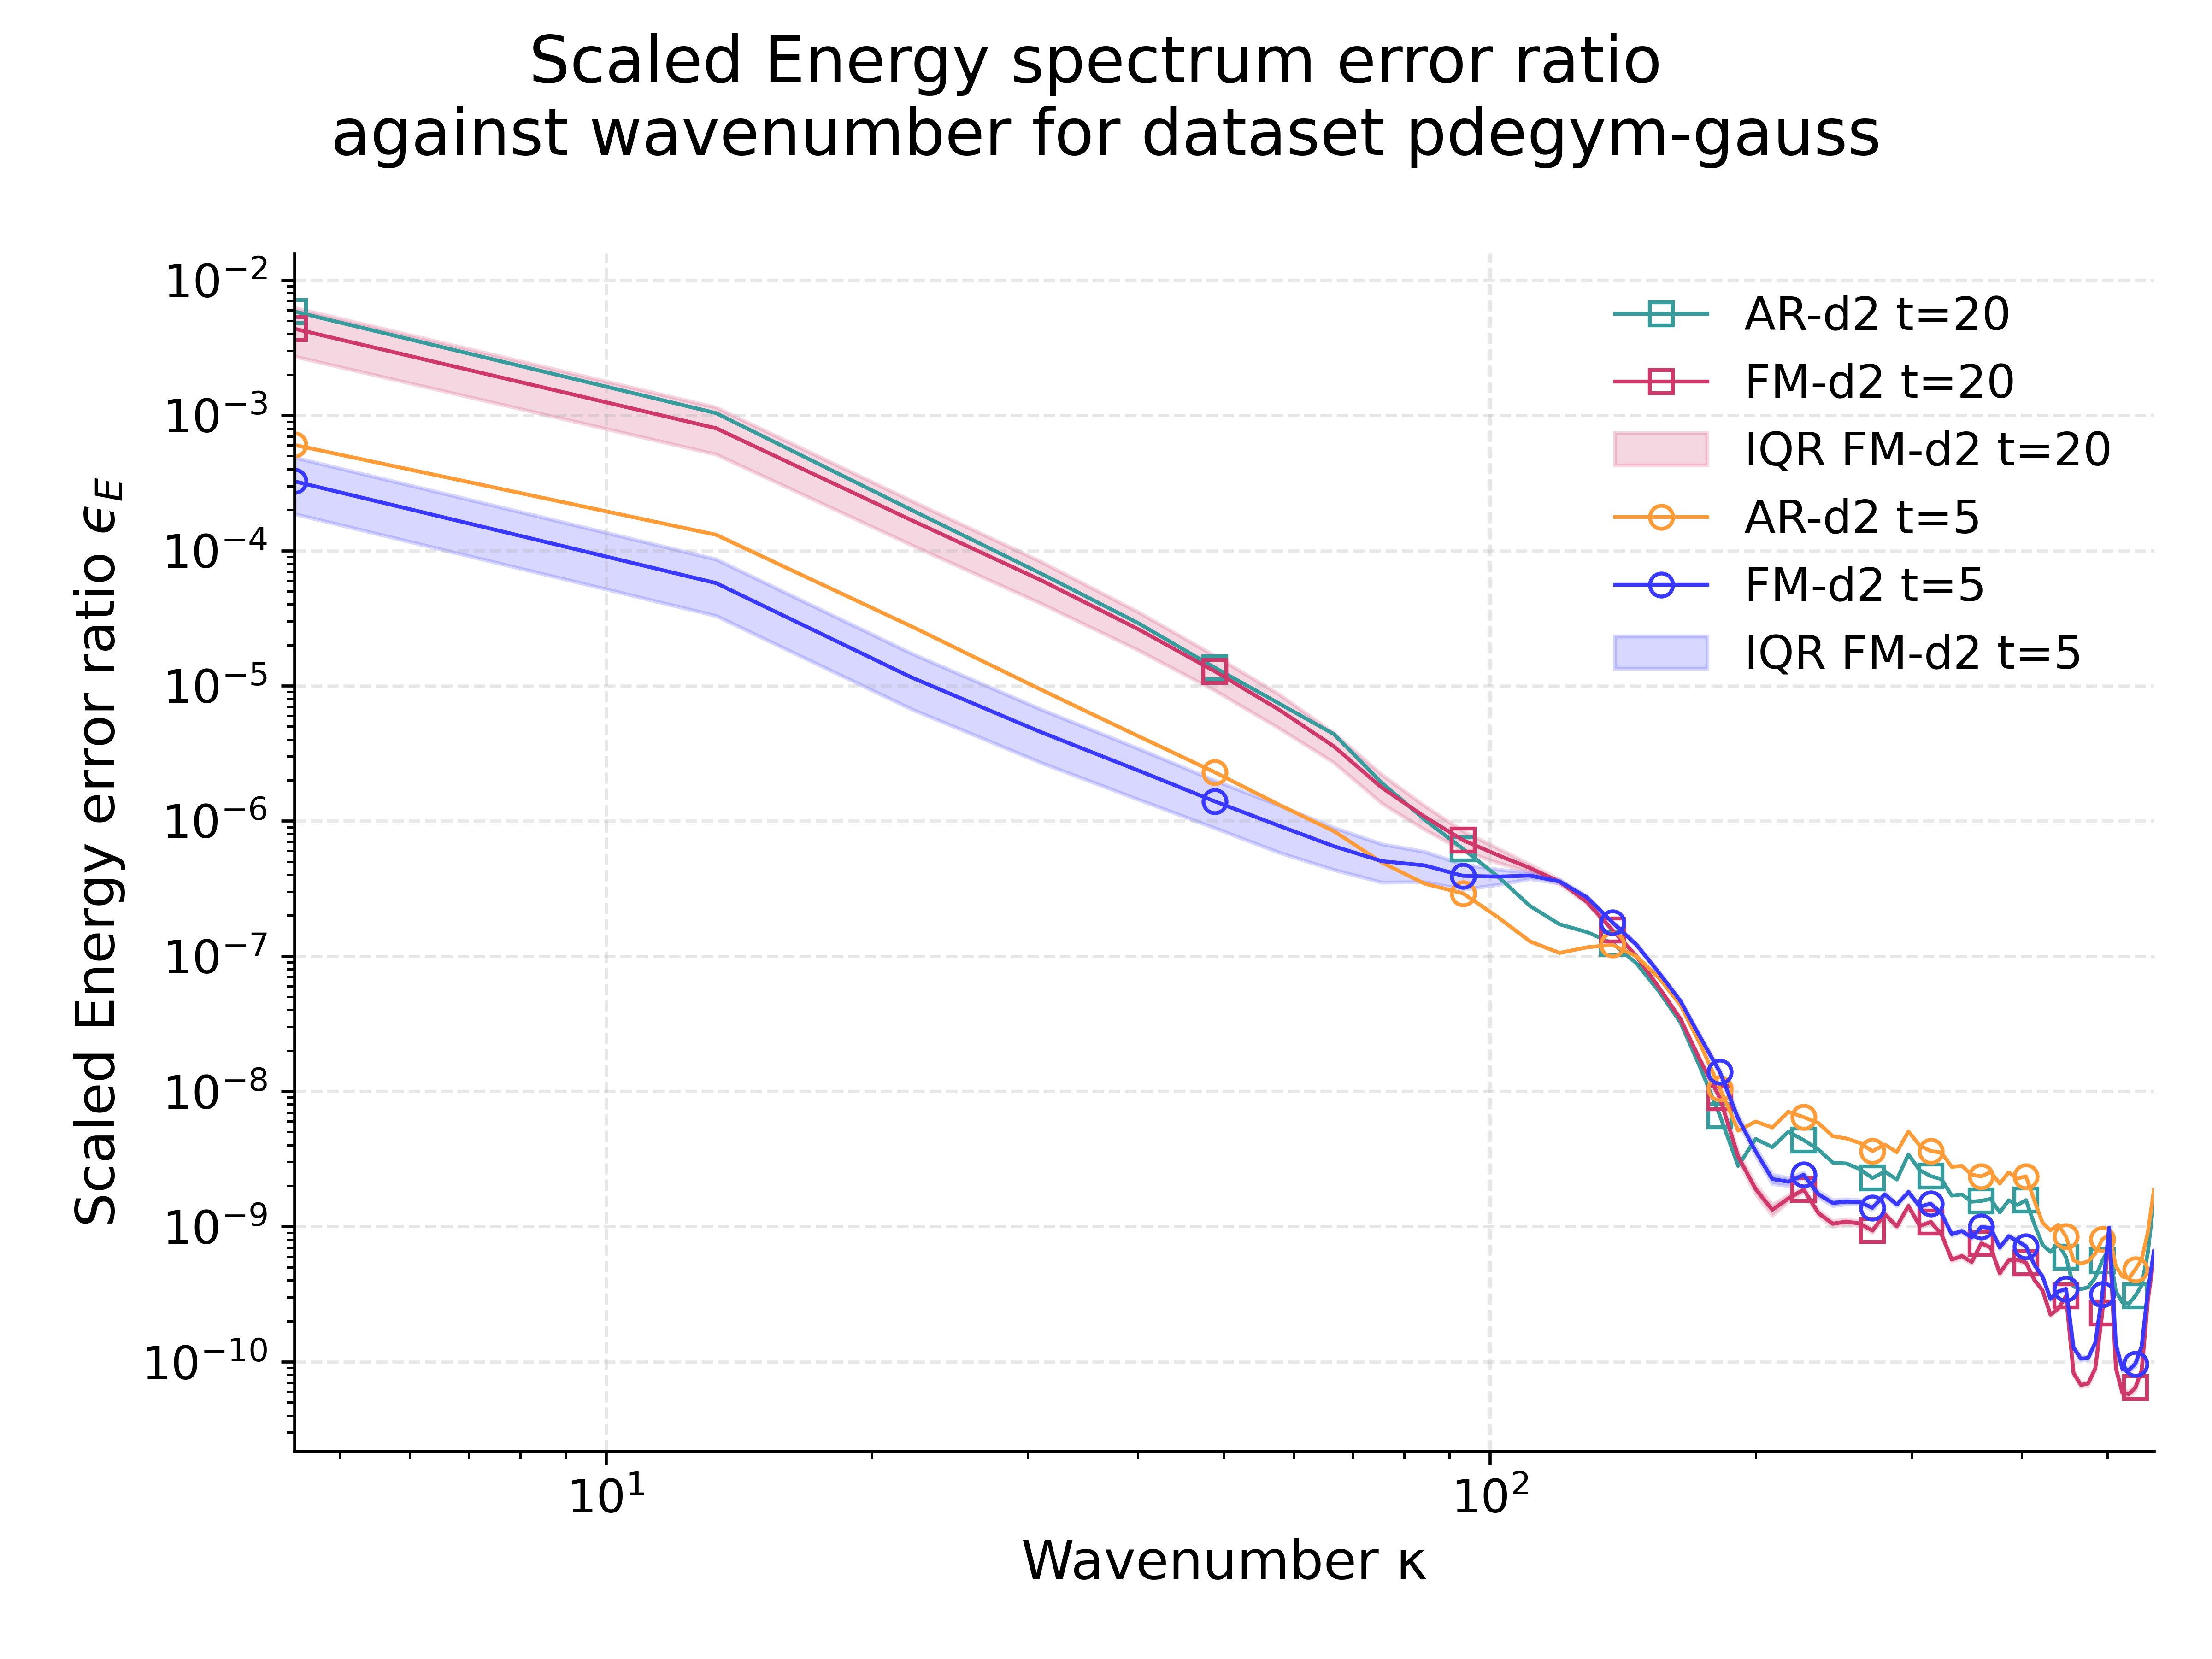
\includegraphics[width=0.8\textwidth]{figs/results/spectra/spectrum_E_pdegym-gauss.png}
    \caption{Scaled energy spectrum error ratio $\epsilon_E$ per wavenumber for the \texttt{pdegym-gauss} dataset, evaluated at $t=5$ and $t=20$.}
    \label{fig:appendix_spectrum_E_pdegym_gauss}
\end{figure}

\begin{figure}[H]
    \centering
    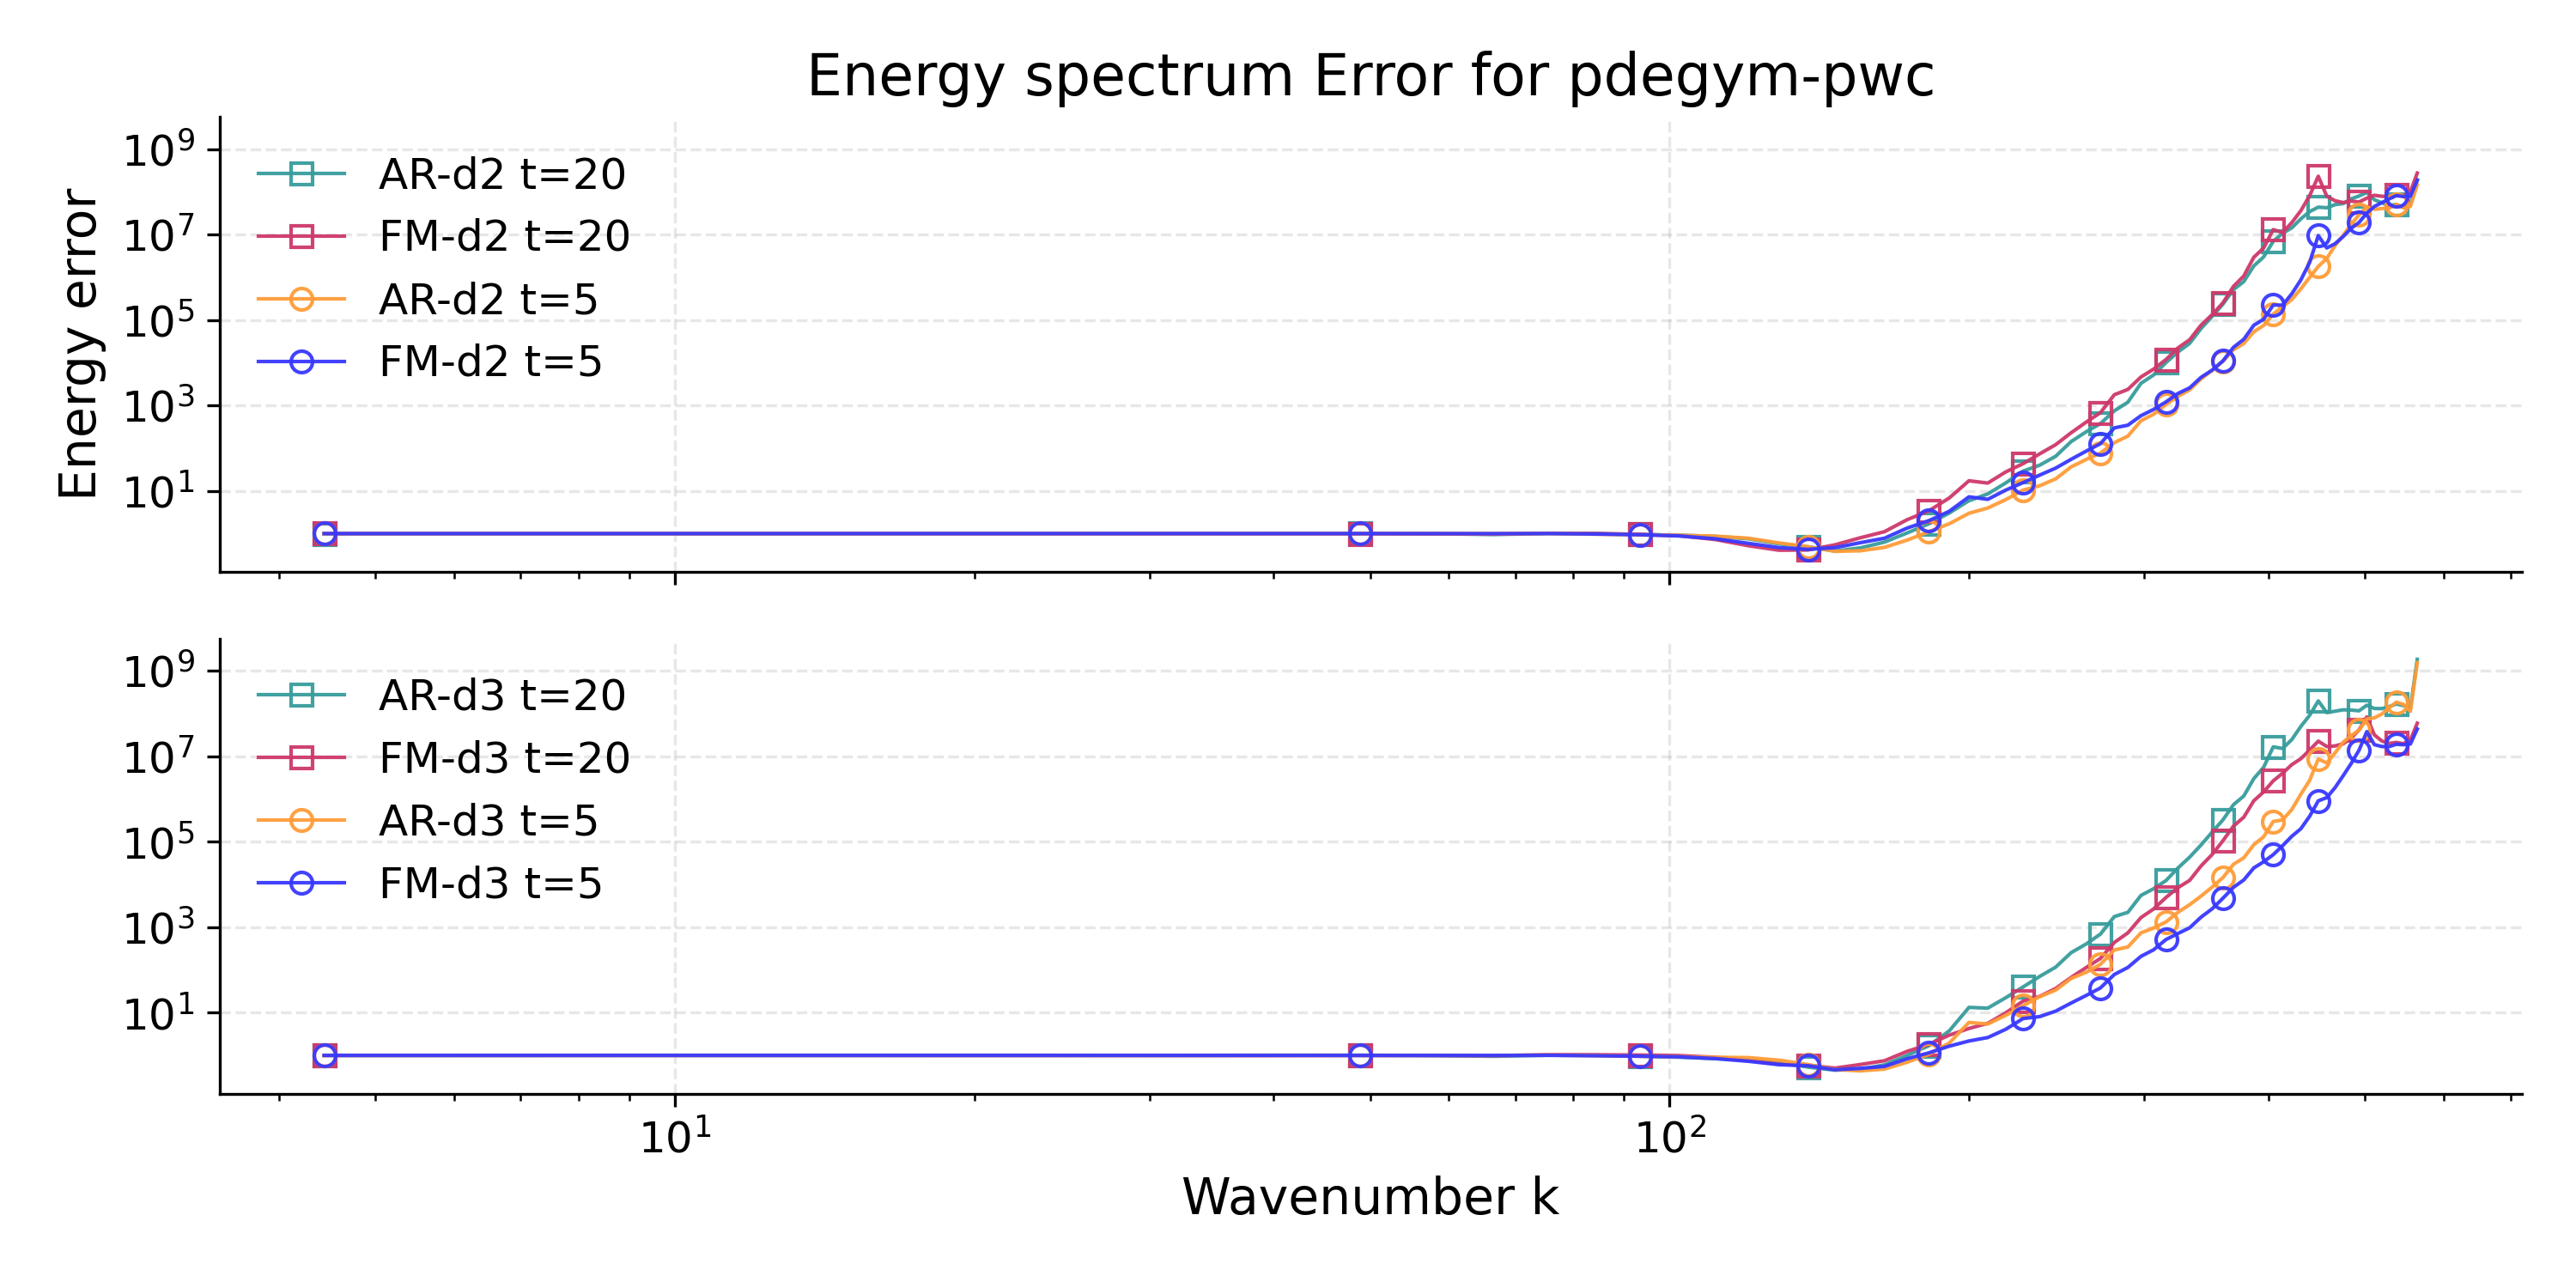
\includegraphics[width=0.8\textwidth]{figs/results/spectra/spectrum_E_pdegym-pwc.png}
    \caption{Scaled energy spectrum error ratio $\epsilon_E$ per wavenumber for the \texttt{pdegym-pwc} dataset, evaluated at $t=5$ and $t=20$.}
    \label{fig:appendix_spectrum_E_pdegym_pwc}
\end{figure}

\begin{figure}[H]
    \centering
    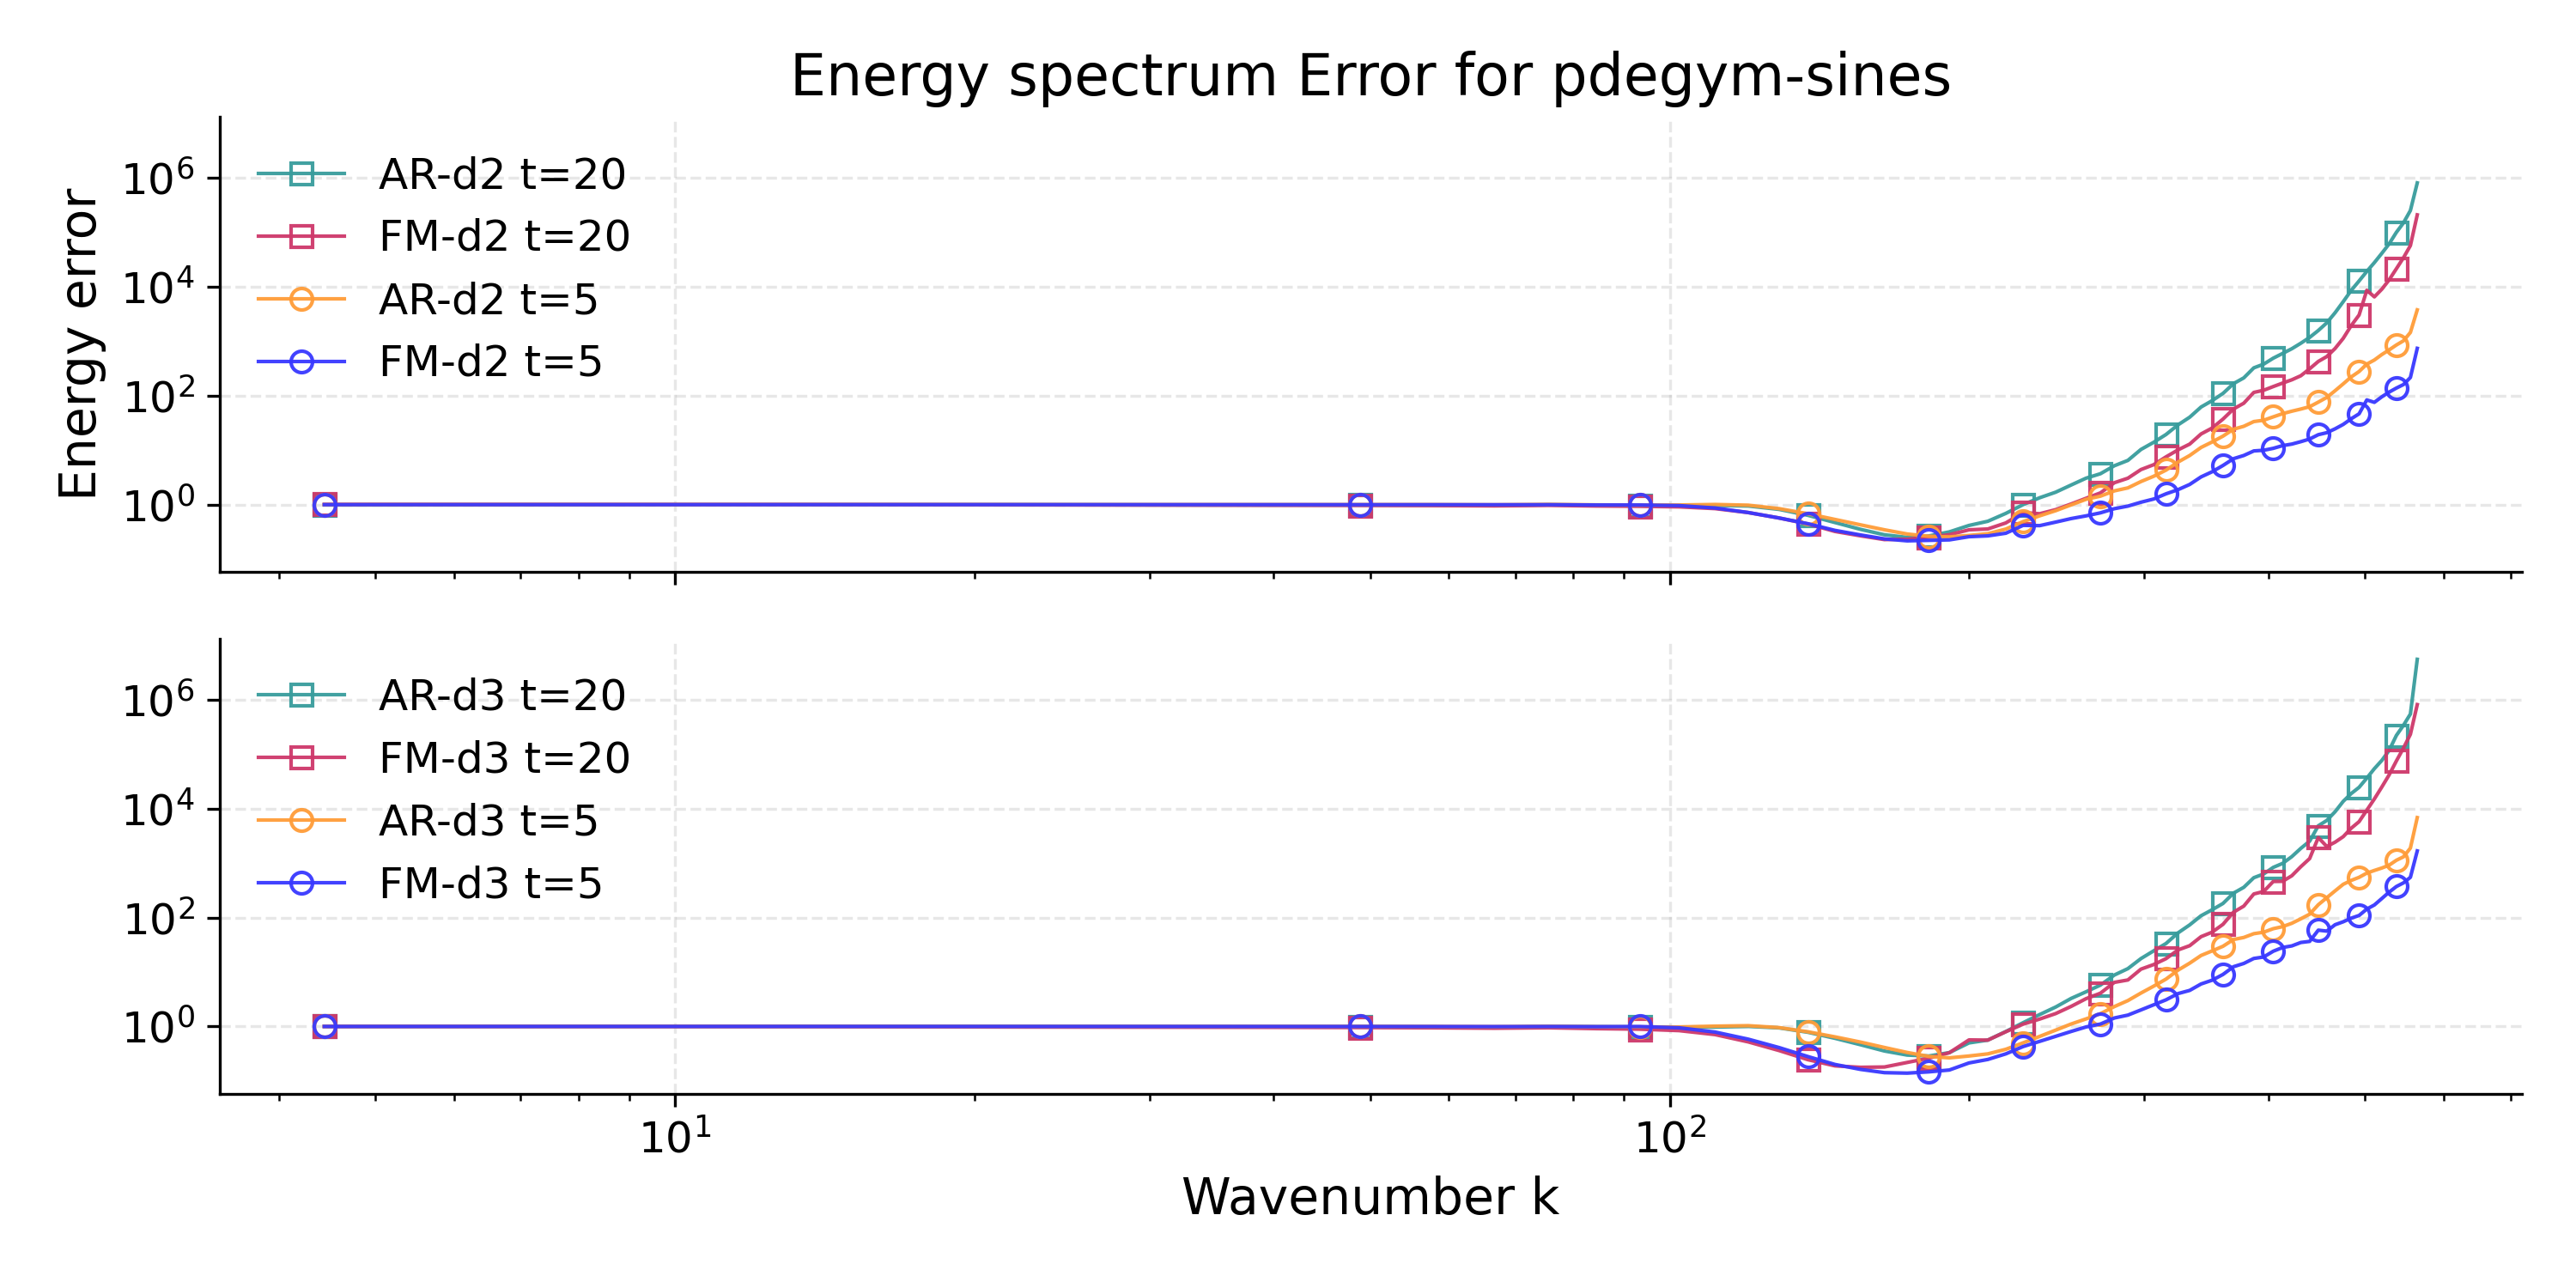
\includegraphics[width=0.8\textwidth]{figs/results/spectra/spectrum_E_pdegym-sines.png}
    \caption{Scaled energy spectrum error ratio $\epsilon_E$ per wavenumber for the \texttt{pdegym-sines} dataset, evaluated at $t=5$ and $t=20$.}
    \label{fig:appendix_spectrum_E_pdegym_sines}
\end{figure}

\begin{figure}[H]
    \centering
    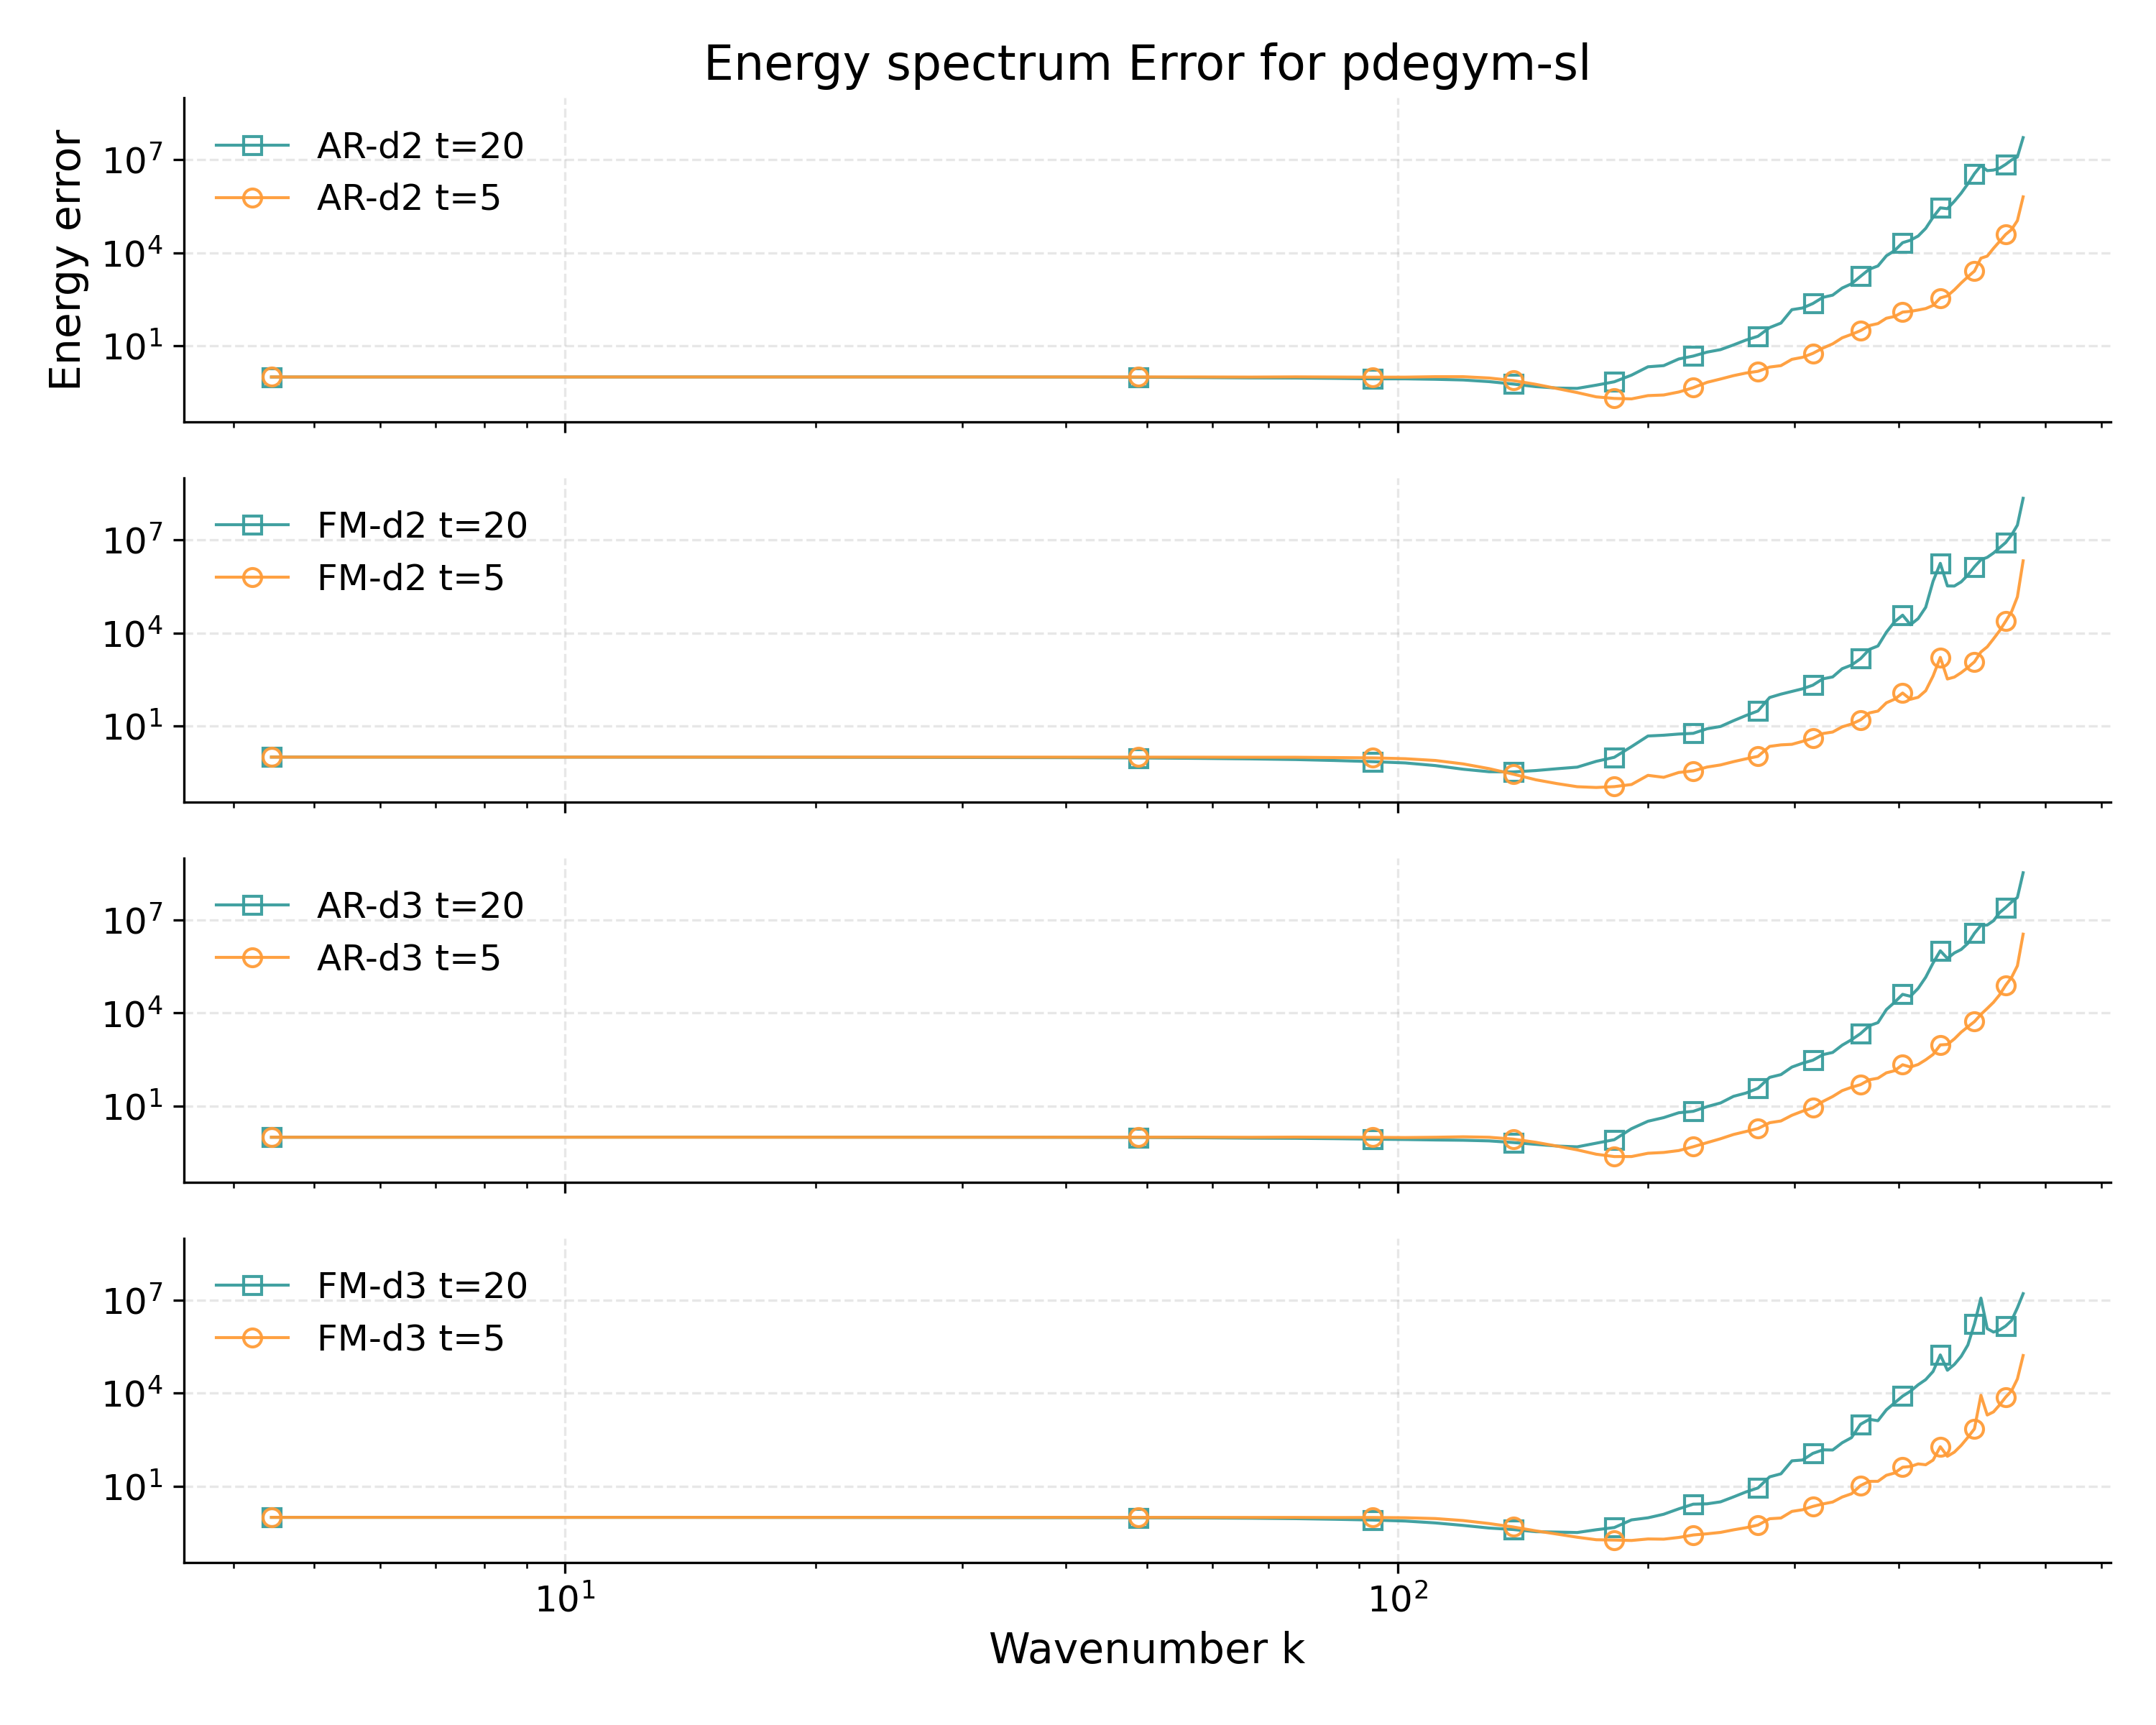
\includegraphics[width=0.8\textwidth]{figs/results/spectra/spectrum_E_pdegym-sl.png}
    \caption{Scaled energy spectrum error ratio $\epsilon_E$ per wavenumber for the \texttt{pdegym-sl} dataset, evaluated at $t=5$ and $t=20$.}
    \label{fig:appendix_spectrum_E_pdegym_sl}
\end{figure}

\begin{figure}[H]
    \centering
    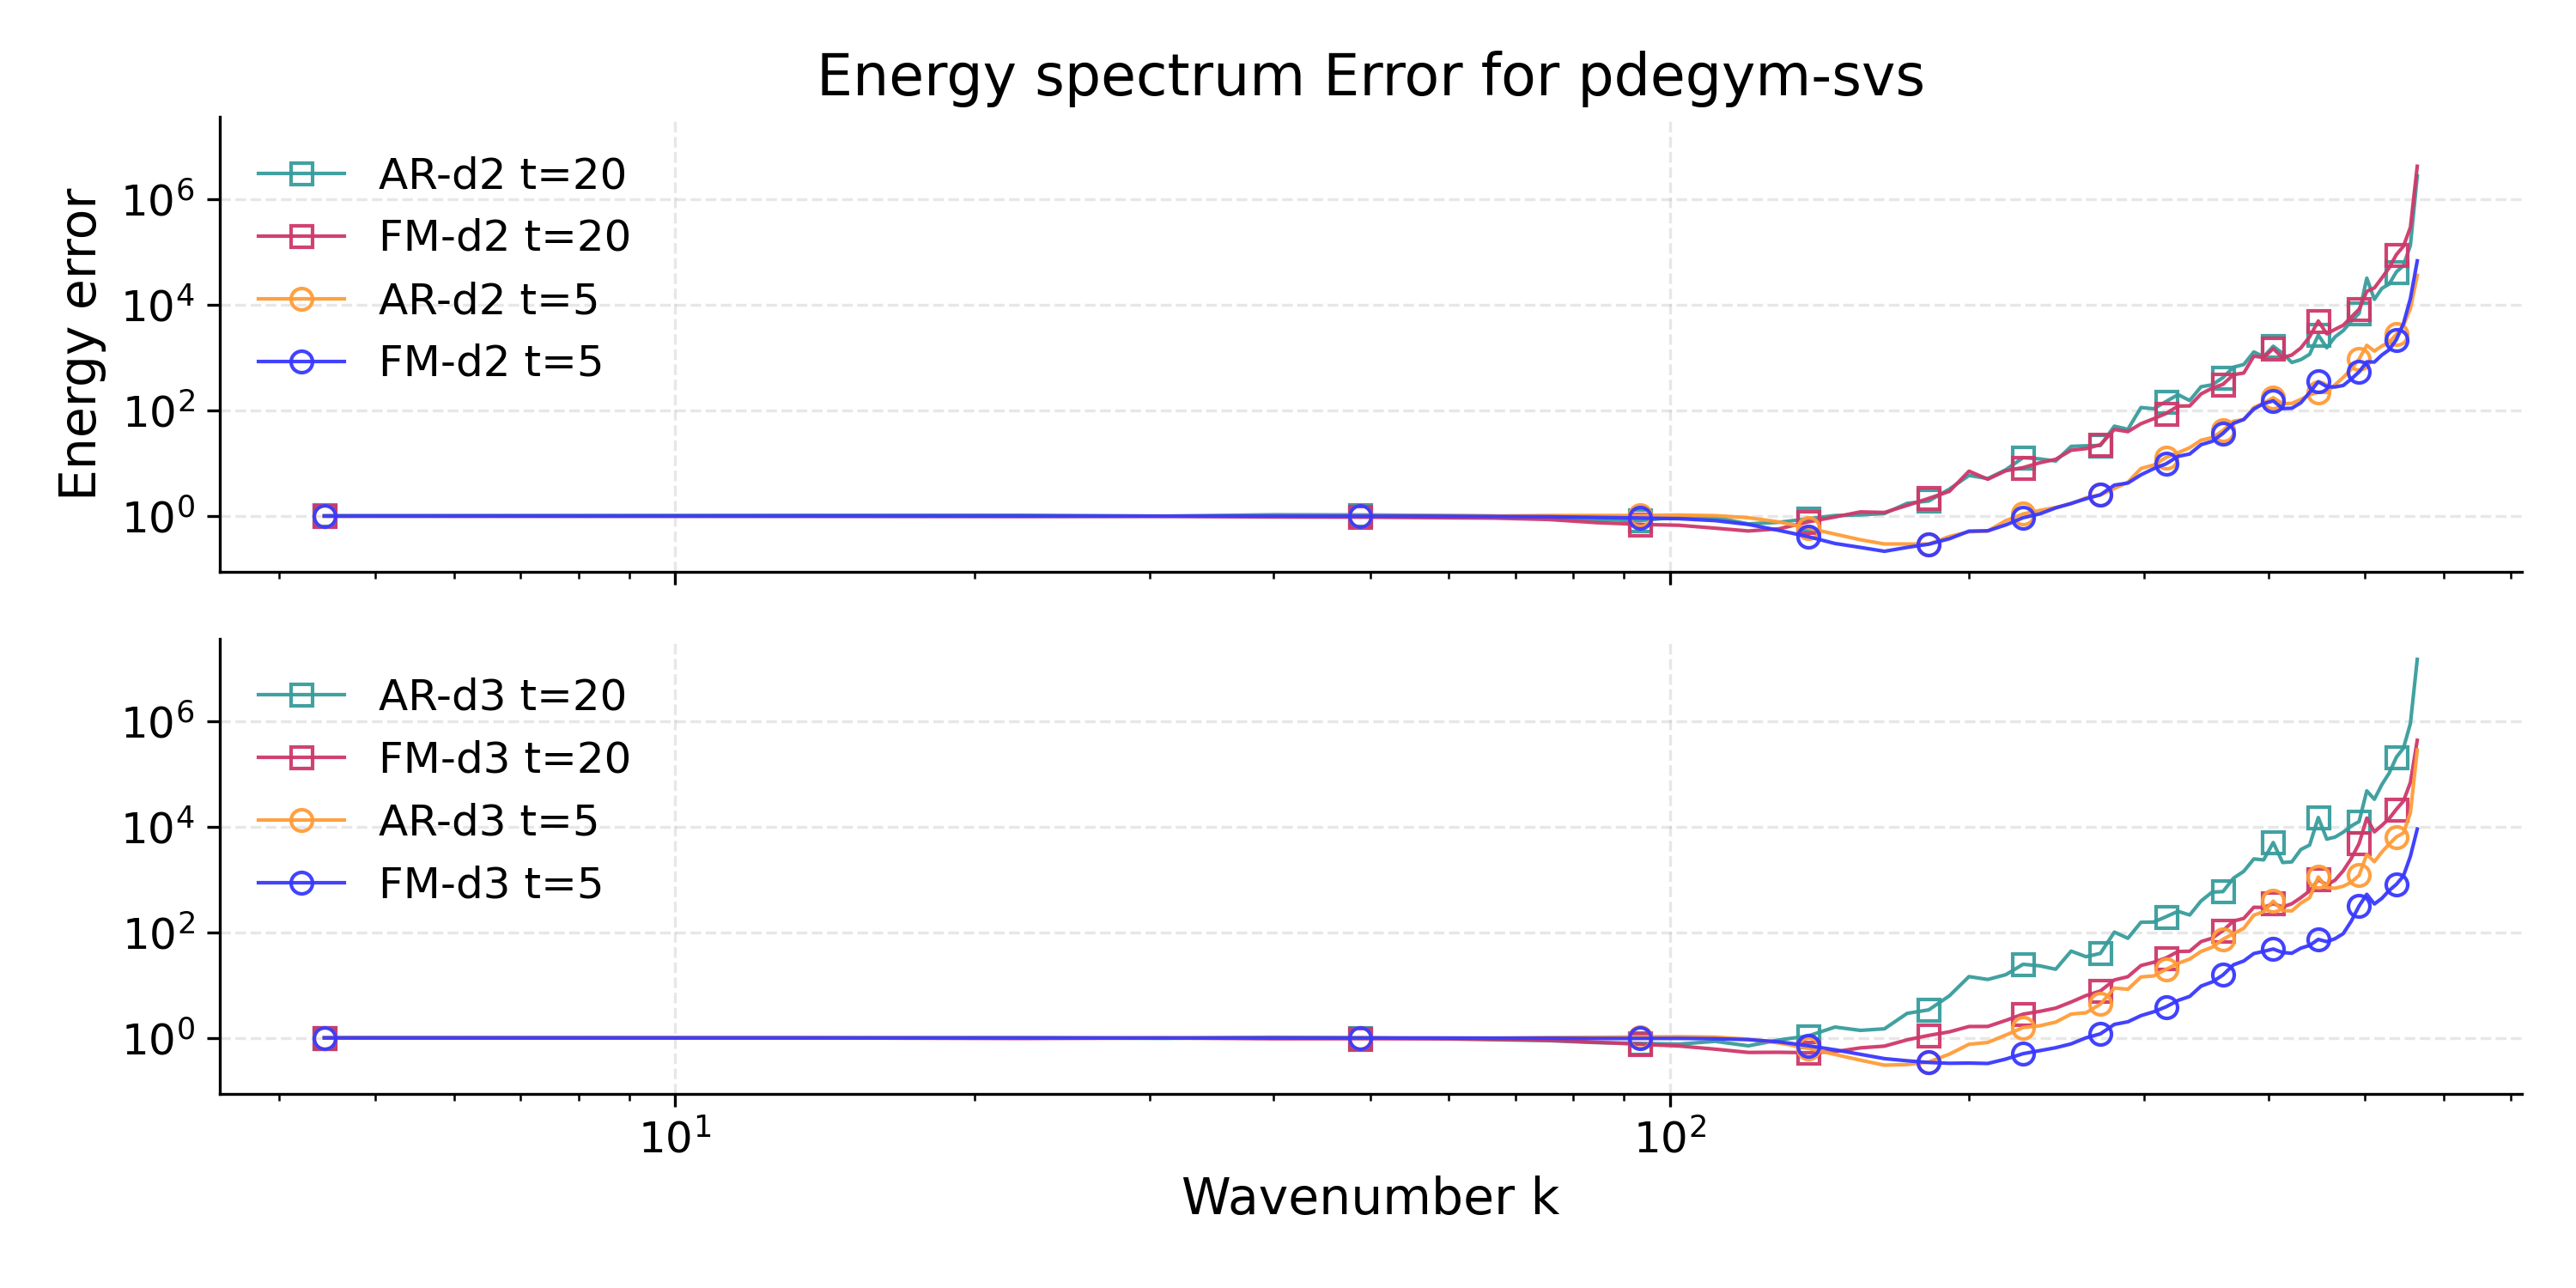
\includegraphics[width=0.8\textwidth]{figs/results/spectra/spectrum_E_pdegym-svs.png}
    \caption{Scaled energy spectrum error ratio $\epsilon_E$ per wavenumber for the \texttt{pdegym-svs} dataset, evaluated at $t=5$ and $t=20$.}
    \label{fig:appendix_spectrum_E_pdegym_svs}
\end{figure}

